\section{Legibilidade da rede ferroviária: revisão a partir de feedback}
\label{sec:legibilidade-ferroviaria}
Em 2 de novembro de 2026, um retorno durante a revisão do aplicativo apontou dificuldade para distinguir o traçado do Metrô e dos trens sobre o mapa, nos temas claro e escuro. O relato mencionou a percepção de cores como possível fator; não foi realizada avaliação clínica nem ensaio com uma amostra de pessoas daltônicas. O problema foi tratado como requisito de legibilidade da interface.

Na revisão atual, os contornos claro e escuro preservam a identificação dos traçados, e os nomes seguem o padrão de modalidade e linha: por exemplo, ``Metrô Linha Verde'' e ``CPTM Linha 12 Safira''. O mapa apresenta no máximo um rótulo por linha visível, afastado do traçado e dos marcadores quando há espaço. A posição do passageiro permanece acima das camadas ferroviárias. Em escalas abrangentes, alguns nomes podem ser omitidos por falta de espaço. As novas capturas mantêm a lâmpada acesa e o mapa colorido; apagar a lâmpada continua sendo uma opção para atenuar os pontos e a base cartográfica.

\begin{figure}[H]\centering
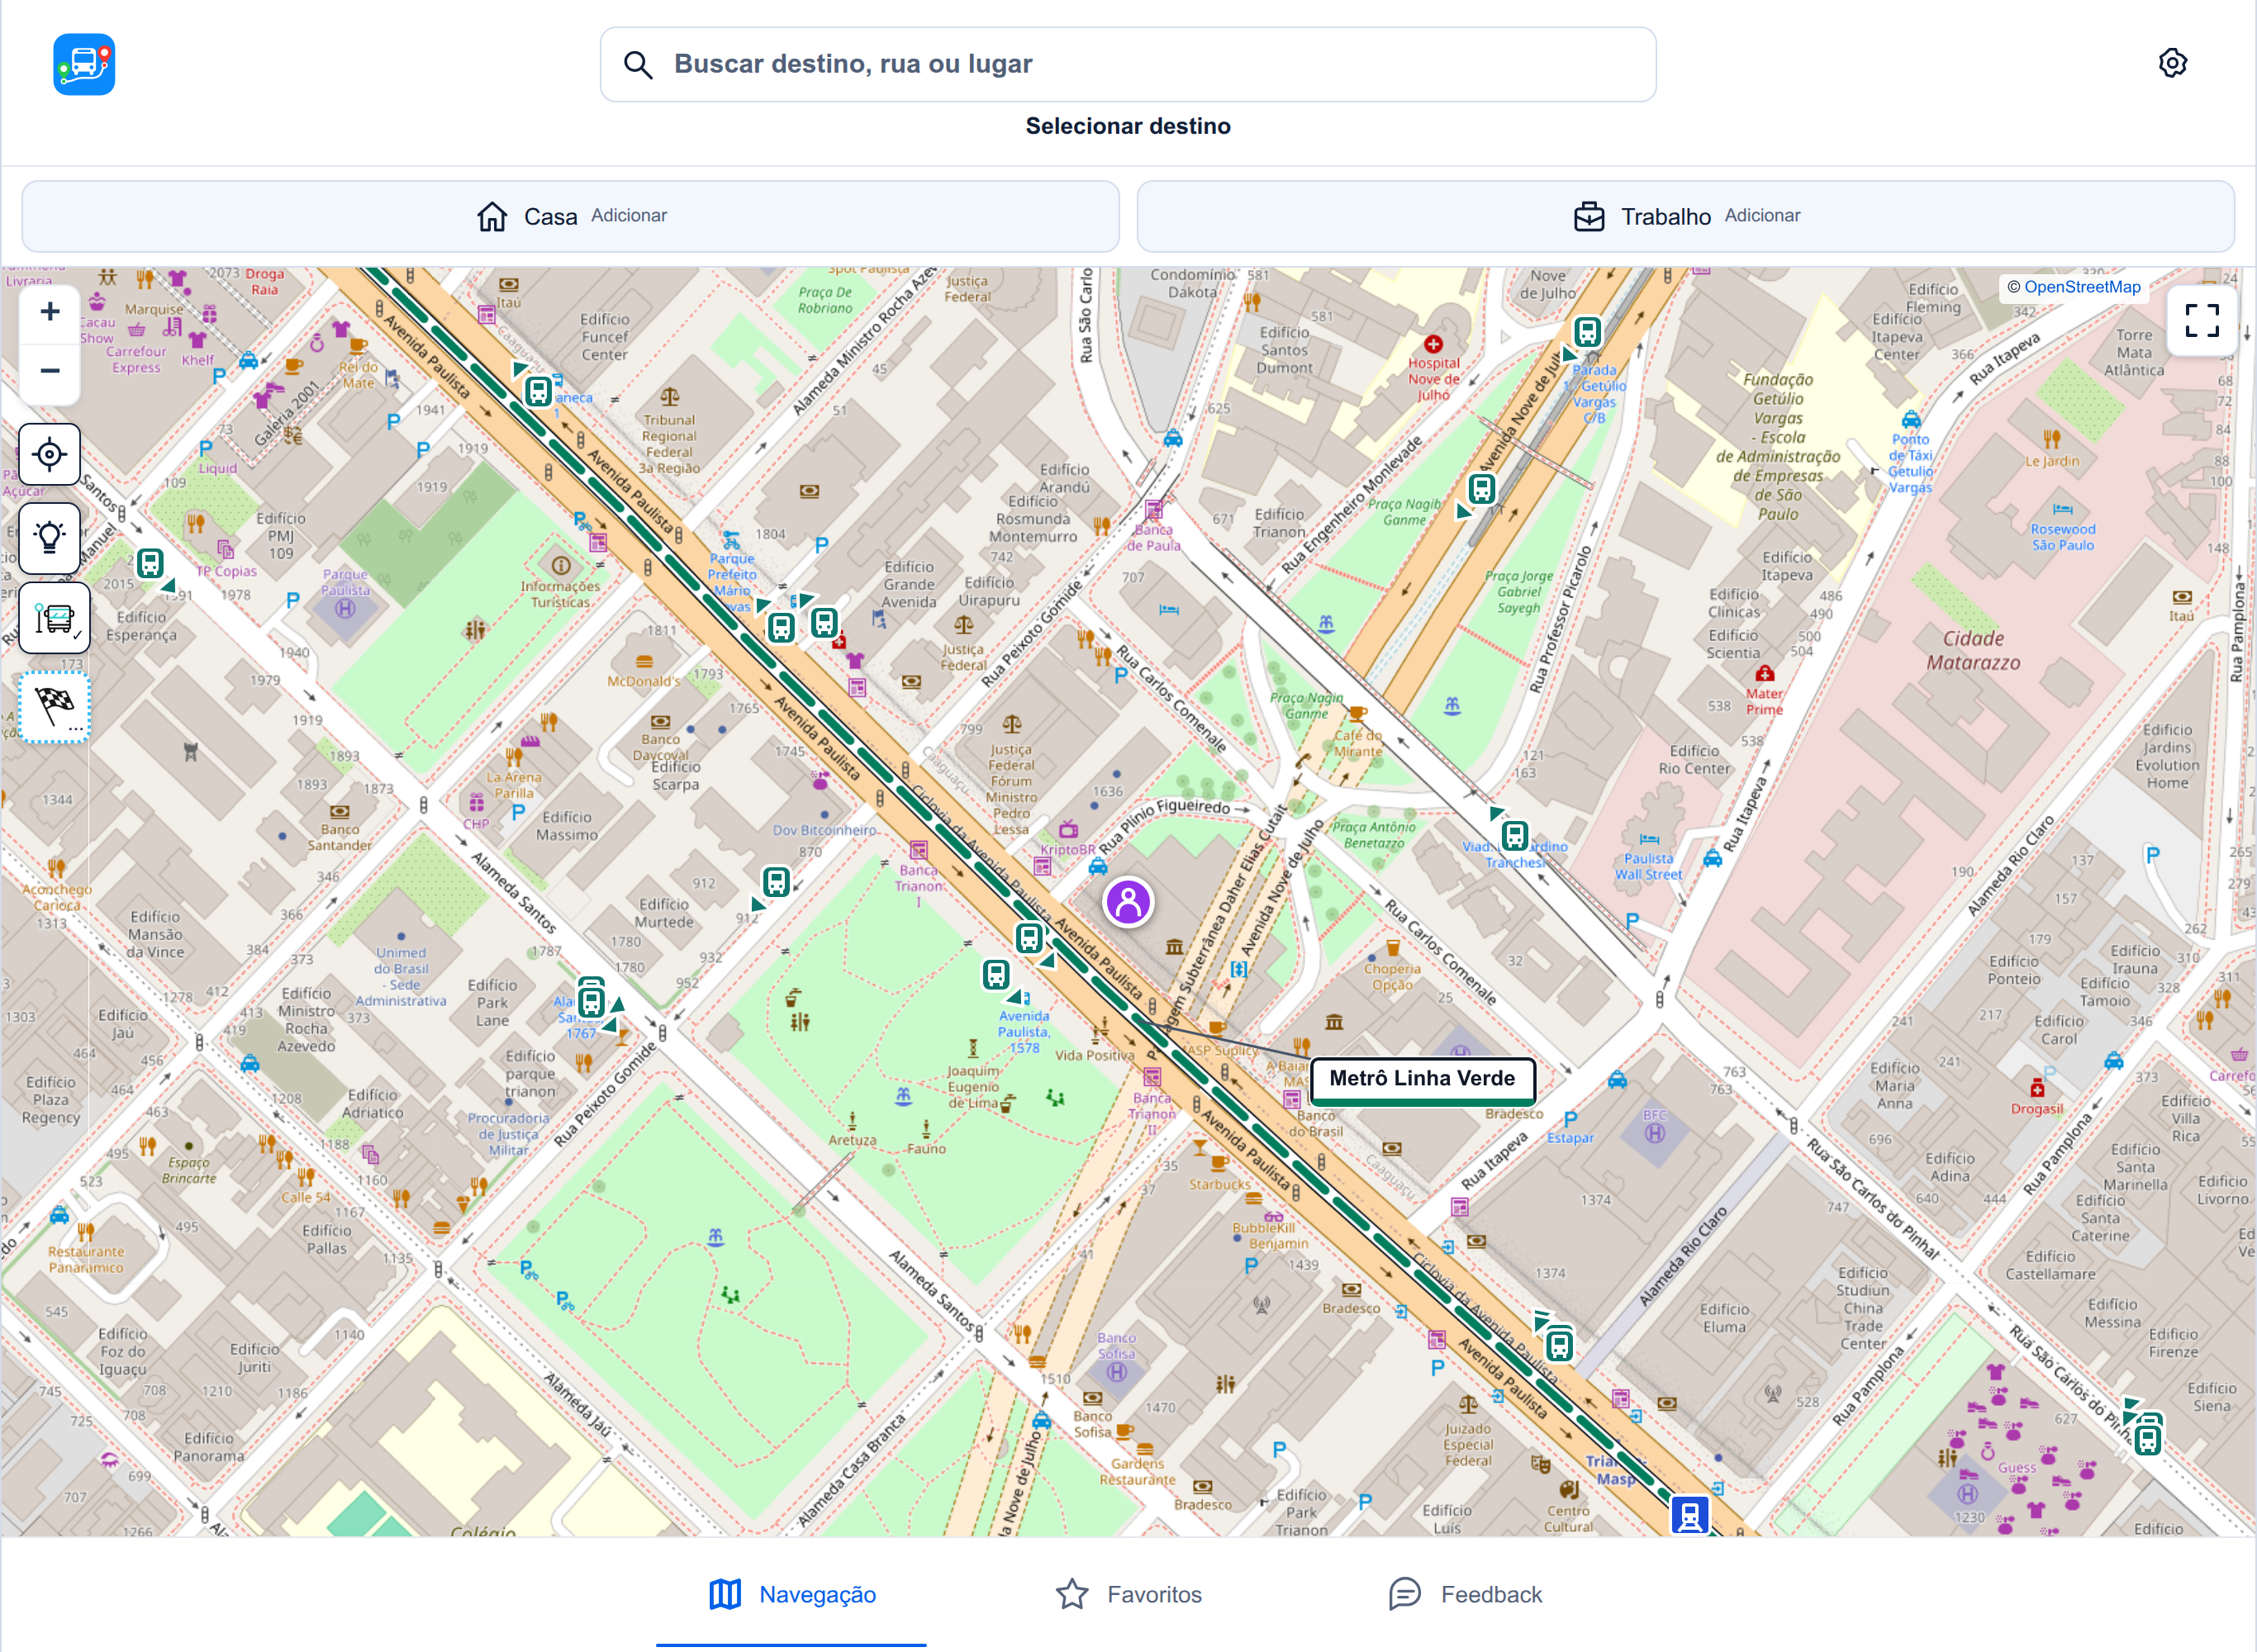
\includegraphics[width=\textwidth,height=0.43\textheight,keepaspectratio]{capturas/2026-11-02-interface-atual/ferrovia-light.png}
\caption{Identificação ferroviária atual no tema claro: mapa colorido e um rótulo para a Linha Verde.}\label{fig:contraste-ferroviario}
\fonte{Captura da revisão 78e3935, 2 nov. 2026; lâmpada acesa e localização simulada no MASP.}
\end{figure}
\begin{figure}[H]\centering
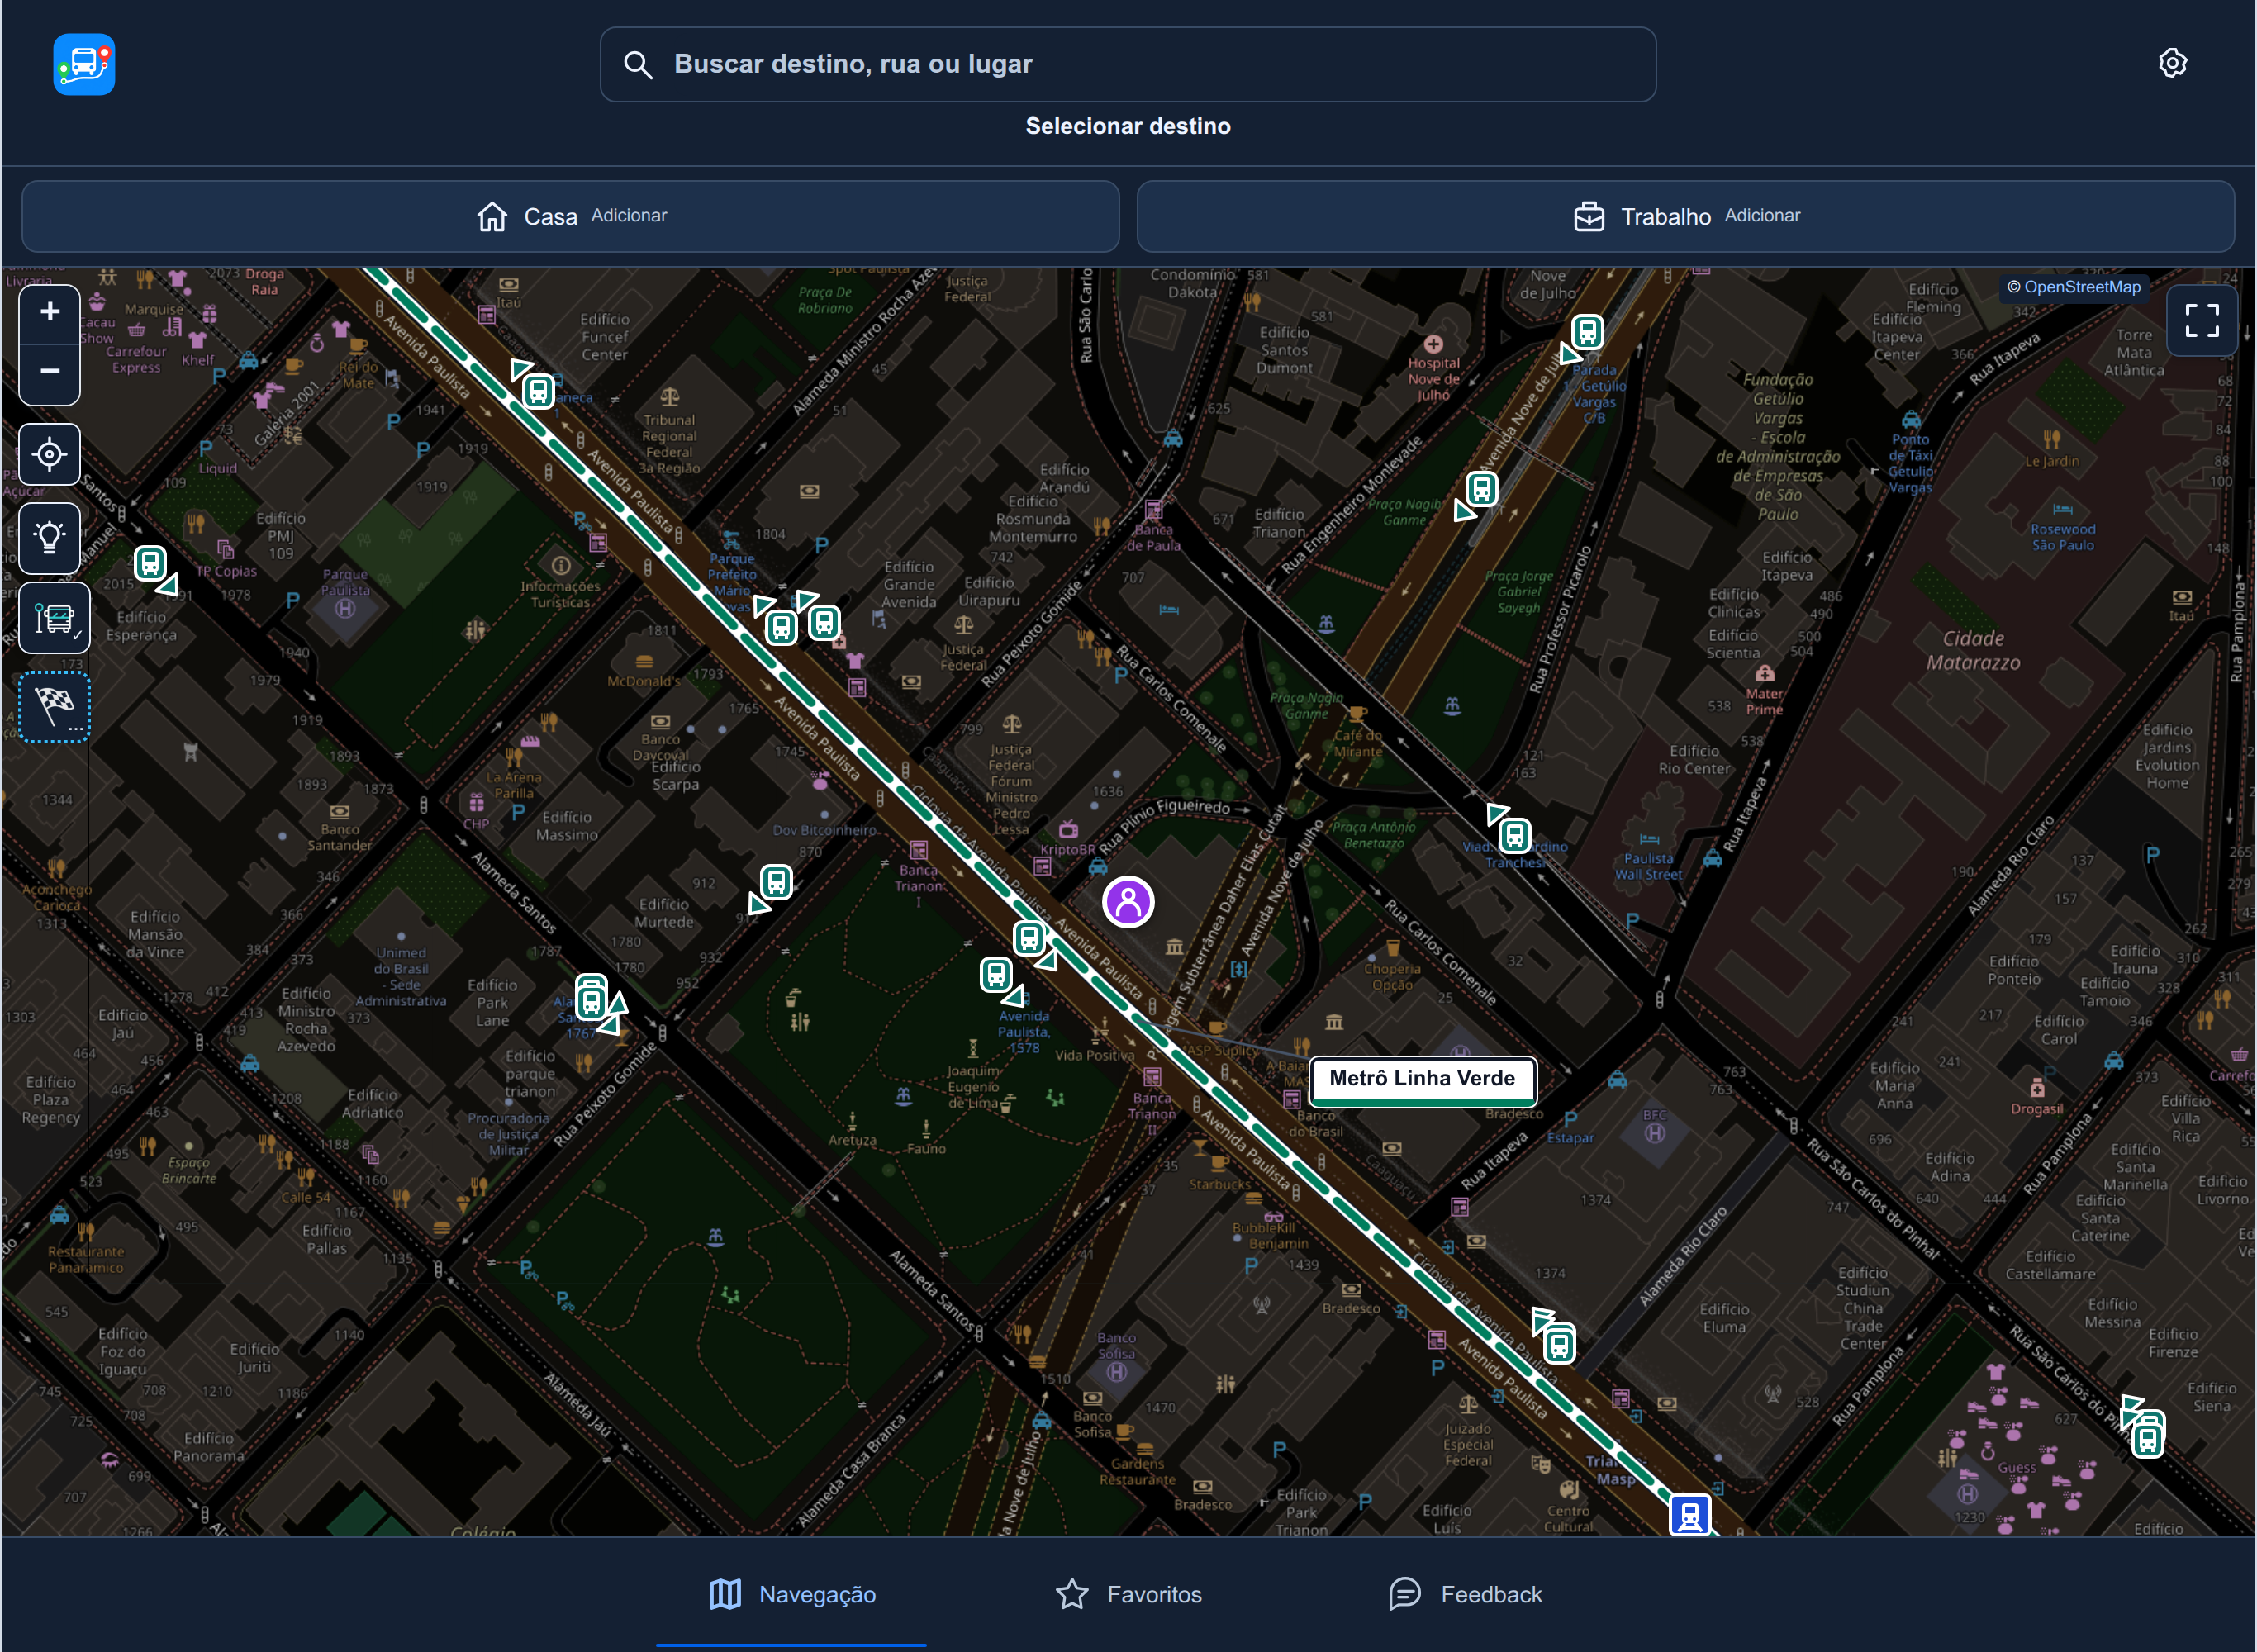
\includegraphics[width=\textwidth,height=0.43\textheight,keepaspectratio]{capturas/2026-11-02-interface-atual/ferrovia-dark.png}
\caption{Identificação ferroviária atual no tema escuro, com o mesmo enquadramento no MASP.}\label{fig:contraste-ferroviario-escuro}
\fonte{Captura da revisão 78e3935, 2 nov. 2026; lâmpada acesa, sem retoque da imagem.}
\end{figure}

A conferência técnica incluiu opacidade, identificadores, mudança de tema, enquadramento e interação com os pontos, além de captura em tela móvel. Os testes automatizados executados não substituem avaliação de compreensão, conforto visual ou acessibilidade com passageiros. Trata-se de correção implementada e verificada tecnicamente, ainda sujeita à avaliação por tarefas prevista para a continuidade do projeto. As Figuras~\ref{fig:contraste-ferroviario} e~\ref{fig:contraste-ferroviario-escuro} documentam a revisão 78e3935 da interface, recapturada em 2 de novembro, sem alterar os resultados históricos dos estudos anteriores.
